\documentclass[UTF8,titlepage]{ctexart}
\usepackage{amsmath,amssymb,amsthm,amsfonts,amscd}
\usepackage{fontspec}
\setmainfont{Times New Roman}
\usepackage{graphicx}
\usepackage{titlesec}
\usepackage{makecell}
\usepackage{longtable}
\usepackage{xcolor}
\usepackage{tcolorbox}
\usepackage{soul}
\usepackage{adjustbox}
\usepackage{tcolorbox}
\usepackage{enumerate}
\usepackage{pdfpages}
\usepackage{float}
\usepackage{colortbl}
\usepackage{tabularx}
\usepackage{multirow}
\usepackage{pgfplots}
\usepackage{minted}
\numberwithin{figure}{section}
\usepackage[left=1.25in,right=1.25in,%
top=1in,bottom=1in]{geometry}
\usepackage{color}
\titleformat{\section}
  {\raggedright\LARGE\bfseries}{\thesection}{1em}{}
\begin{document}
\title{{\Huge{\textbf{程序设计实践报告}}}}
\author{姓名:赵伯远 \\ 学号:211440128 \\班级:人工智能2101 \\ 序号:75}
\date{\today}
\maketitle
\tableofcontents
\clearpage

\section{课题一:运动会分数统计}

\subsection{任务描述}

参加运动会有 n 个学校,学校编号为 1……n。比赛分成m 个男子项目和w个女子项目。项目编号为男子:1$\sim$m,女子:m+1$\sim$m+w。不同的项目取前五名或前三名积分;取前五名的积分分别为:7、5、3、2、1,前三名的积分分别为:5、3、2;哪些项目取前五名或前三名由学生自己设定。(m<=20, n<=20)
 
\subsection{功能要求}

\begin{enumerate}
    \item 可以输入各个项目的前三名或前五名的成绩;
    \item 能统计各学校总分;
    \item 可以按学校编号、学校总分、男女团体总分排序输出;
    \item 可以按学校编号查询学校某个项目的情况;
    \item 可以按项目编号查询取得前三或前五名的学校。
    \item 允许用户指定某项目采取其他名次的取法。
    \end{enumerate}

\subsection{需求分析}
此程序主要实现的功能有:
\begin{enumerate}
    \item 收集每个学校的男女团队在各项目中的得分。
    \item 按照学校编号、总分、男女团体得分进行排序。
    \item 提供查询功能:查询指定学校在指定项目中的得分,查询指定项目取得前几名的学校。
\end{enumerate}

首先需要构建顺序表储存相关信息,如参赛学校的名称,获得的分数,比赛
项目,及其相关的赋分规则,以及参赛选手信息。然后需要输入比赛相关信息,
如参数学校,比赛项目的相关信息,至此基础信息完备。在项目结束后输入相关
获奖人员信息即可按照积分给出各种排名。

程序流程图如下:
\begin{figure}[H]
\centering
 \resizebox{0.5\textwidth}{!}{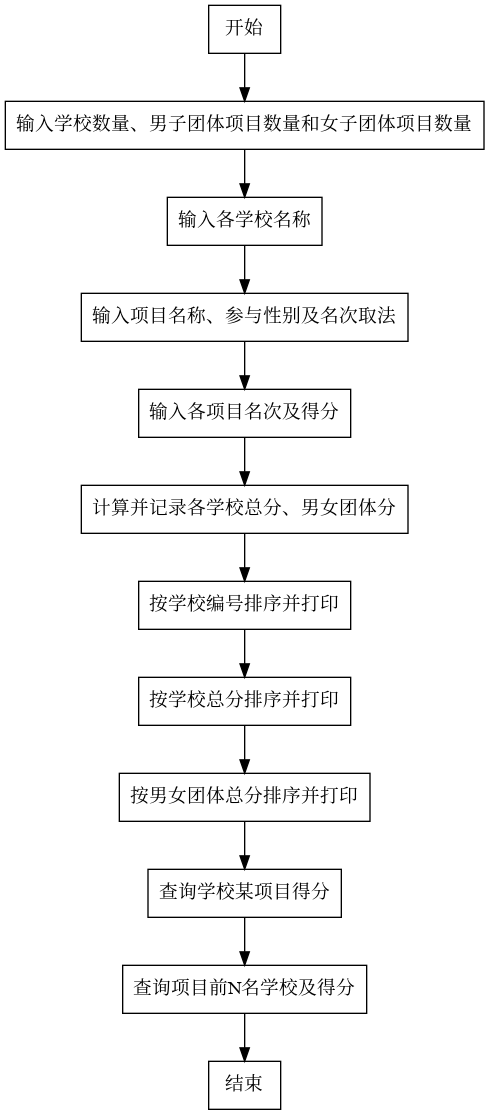
\includegraphics{./fig/program_flowchart.png}}
 \caption{程序流程图}
 \label{}
\end{figure}

\subsection{概要分析}
\begin{figure}[H]
\centering
 \resizebox{1\textwidth}{!}{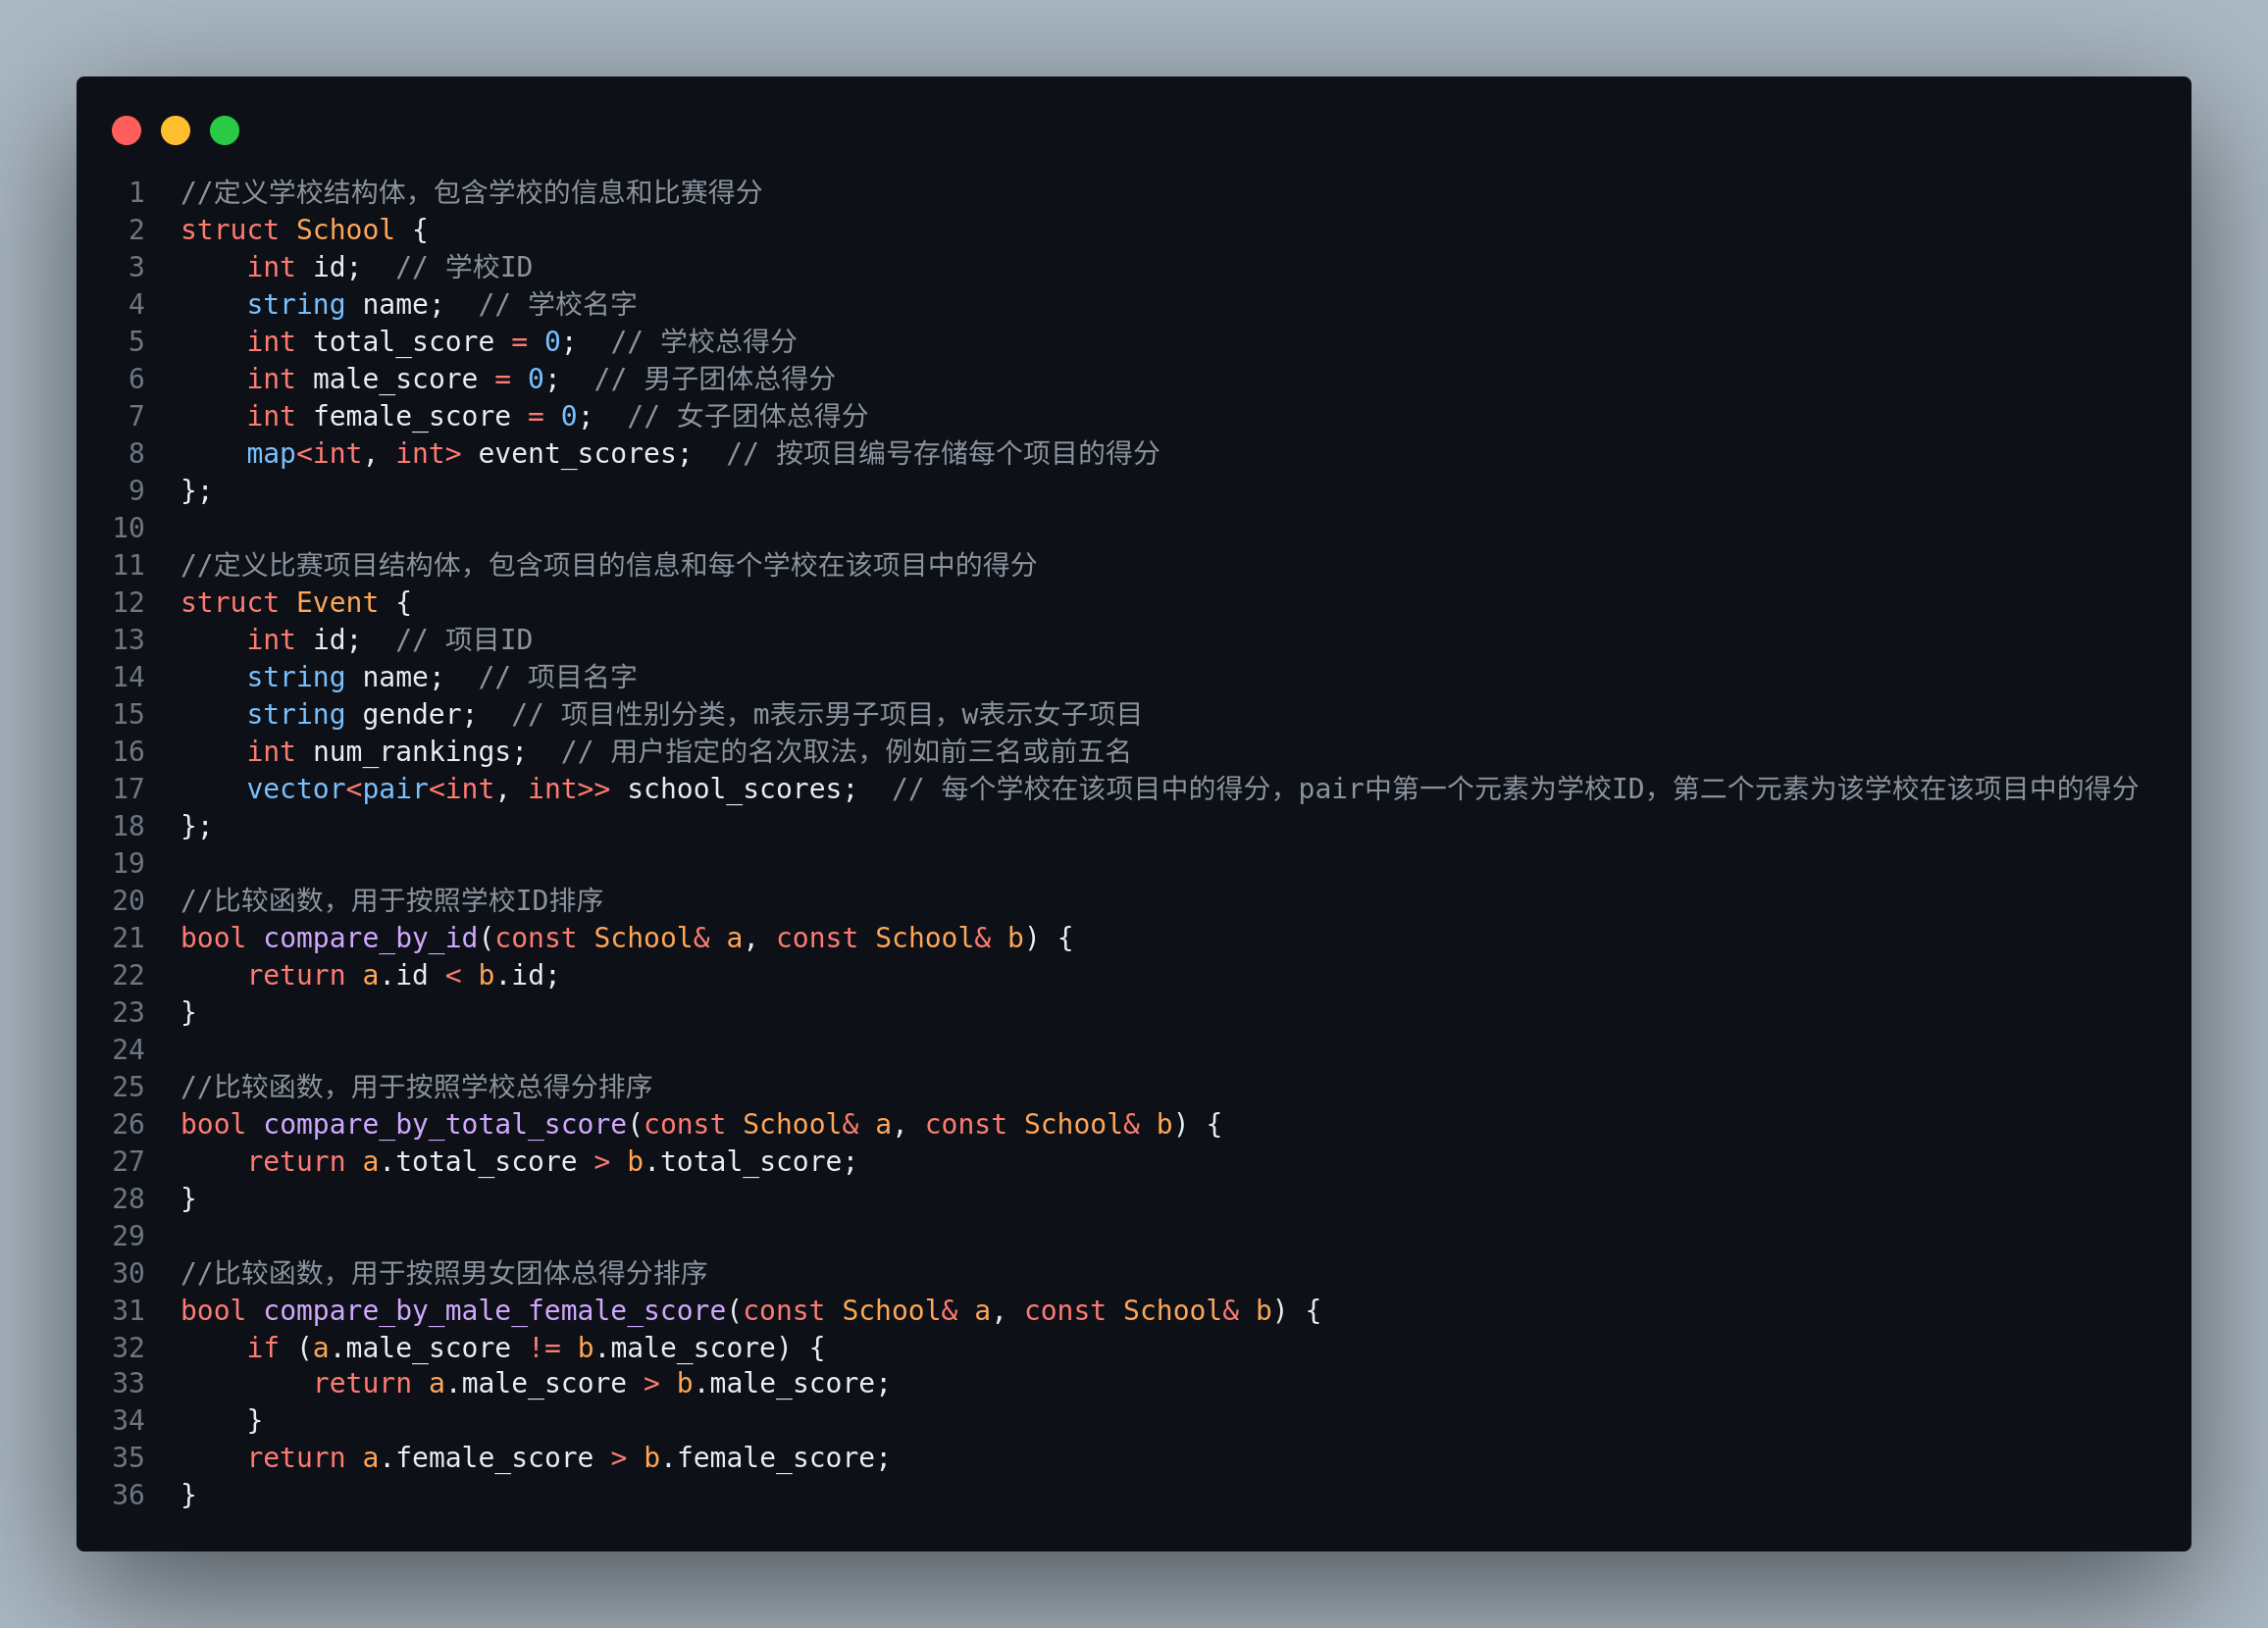
\includegraphics{./fig/struct.png}}
 \caption{程序基本结构体\&基本函数}
 \label{}
\end{figure}

\subsection{详细分析}
完整代码如下:
\begin{minted}{c++}
#include <iostream>
#include <vector>
#include <map>
#include <algorithm>
#include <string>

using namespace std;

//定义学校结构体,包含学校的信息和比赛得分
struct School {
    int id;  // 学校ID
    string name;  // 学校名字
    int total_score = 0;  // 学校总得分
    int male_score = 0;  // 男子团体总得分
    int female_score = 0;  // 女子团体总得分
    map<int, int> event_scores;  // 按项目编号存储每个项目的得分
};

//定义比赛项目结构体,包含项目的信息和每个学校在该项目中的得分
struct Event {
    int id;  // 项目ID
    string name;  // 项目名字
    string gender;  // 项目性别分类,m表示男子项目,w表示女子项目
    int num_rankings;  // 用户指定的名次取法,例如前三名或前五名
    vector<pair<int, int>> school_scores;  // 每个学校在该项目中的得分,
                                           //pair中第一个元素为学校ID,
                                           //第二个元素为该学校在该项目中的得分
};

//比较函数,用于按照学校ID排序
bool compare_by_id(const School& a, const School& b) {
    return a.id < b.id;
}

//比较函数,用于按照学校总得分排序
bool compare_by_total_score(const School& a, const School& b) {
    return a.total_score > b.total_score;
}

//比较函数,用于按照男女团体总得分排序
bool compare_by_male_female_score(const School& a, const School& b) {
    if (a.male_score != b.male_score) {
        return a.male_score > b.male_score;
    }
    return a.female_score > b.female_score;
}


int main() {
    int n, m, w;
    cout << "请输入学校数量、男子团体项目数量、女子团体项目数量:" << endl;
    cin >> n >> m >> w;
    cout << "请输入学校名称:" << endl;
    vector<School> schools(n);
    for (int i = 0; i < n; ++i) {
        schools[i].id = i + 1;
        cin >> schools[i].name;
    }
    cout << "请输入项目名称, 参与性别及名次取法:" << endl; // 让用户指定每个项目的名次取法
    vector<Event> events(m + w);
    for (int i = 0; i < m + w; ++i) {
        events[i].id = i + 1;
        // 获取用户指定的名次取法
        cin >> events[i].name >> events[i].gender 
            >> events[i].num_rankings; 
    }

    for (auto& event : events) {
        for (int i = 0; i < event.num_rankings; ++i) { // 根据用户指定的名次取法计算学校得分
            int school_id, score;
            cout<< "请输入项目 " << event.name << " 的第 " 
                << i + 1 << " 名学校编号和得分:" << endl;
            cin >> school_id >> score;
            event.school_scores.push_back({school_id, score});

            School& school = schools[school_id - 1];
            school.total_score += score;
            if (event.gender=="m") {
                school.male_score += score;
            } else {
                school.female_score += score;
                cout<< school.female_score<<endl;
            }
            school.event_scores[event.id] = score;
        }
    }
    // 输出学校编号排序
    sort(schools.begin(), schools.end(), compare_by_id);
    cout << "按学校编号排序:" << endl;
    for (const auto& school : schools) {
        cout << school.name << " (编号: " << school.id << ")" << endl;
    }
    cout << endl;

    // 输出学校总分排序
    sort(schools.begin(), schools.end(), compare_by_total_score);
    cout << "按学校总分排序:" << endl;
    for (const auto& school : schools) {
        cout << school.name << " (总分: " << school.total_score << ")" << endl;
    }
    cout << endl;

    // 输出男女团体总分排序
    sort(schools.begin(), schools.end(), compare_by_male_female_score);
    cout << "按男女团体总分排序:" << endl;
    for (const auto& school : schools) {
        cout << school.name << " (男子团队分数: " << school.male_score 
             << ", 女子团队分数: " << school.female_score << ")" << endl;
    }
    cout << endl;

    // 查询学校某个项目的情况
    int query_school_id, query_event_id;
    cout << "请输入查询的学校编号和项目编号:" << endl;
    cin >> query_school_id >> query_event_id;
    const School& query_school = schools[query_school_id - 1];
    auto it = query_school.event_scores.find(query_event_id);
    if (it != query_school.event_scores.end()) {
        cout << query_school.name << " 在项目 " << events[query_event_id - 1].name 
             << " 中的得分为: " << it->second << endl;
    } else {
        cout << query_school.name << " 在项目 " << events[query_event_id - 1].name 
             << " 中没有得分" << endl;
    }
    cout << endl;

    // 按项目编号查询取得前三或前五名的学校
    cout << "请输入要查询的项目编号:" << endl;
    int query_event_id2;
    cin >> query_event_id2;
    const Event& query_event = events[query_event_id2 - 1];

    cout << "在项目 " << query_event.name << " 中取得前" 
         << query_event.num_rankings << "名的学校有:" << endl;
    for (const auto& school_score : query_event.school_scores) {
        cout << schools[school_score.first - 1].name << " (得分: " 
             << school_score.second << ")" << endl;
    }

    return 0;
}


\end{minted}

\subsection{调试分析}
\begin{enumerate}
    \item 问题:在计算学校得分时,学校编号的索引与实际编号存在偏差。
    
          解决方案:在读取学校编号后,需要将其减1,以符合实际索引。
    

          \item 问题:按学校编号排序输出时,学校编号不是按照升序排列。
    
          解决方案:可以在排序函数sort(schools.begin(), schools.end(), compare\_by\_id)之前添加调用compare\_by\_id函数的输出语句,检查是否正确比较学校编号。
    \item 问题:程序无法正确查询取得前三或前五名的学校。
    
          解决方案:根据用户输入的项目编号,获取该项目的参与学校列表,并根据学校的得分进行排序。然后输出前三或前五名学校的名称和得分。确保在处理边界情况时进行适当的错误检查。

\end{enumerate}

\subsection{用户手册}
\begin{enumerate}
    \item 演示程序的运行环境为 Ubuntu 20.04 系统,GCC 9.4.0\ x86\_64-linux-gnu.。执行指令为
    
    cd "/media/zby/SSD数据盘/Program-Practice/Sport/" \&\& g++ main.cpp -o main \&\& "/media/zby/SSD数据盘/Program-Practice/Sport/"main


\end{enumerate}

\section{课题三:迷宫问题}

\subsection{任务描述}
迷宫问题是取自心理学的一个古典实验。实验中,把一只老鼠从一个没有顶
的大盒子的门放入,在盒中设置了许多墙,对行进的方向形成了多处阻挡。盒子
仅仅有一个出口,在出口处放置了一块奶酪,吸引老鼠在迷宫中寻找道路以到达
出口。重复对老鼠进行上述实验,看老鼠能在多久找到出口。
请设计一个算法实现迷宫问题求解。

\subsection{功能要求}

找到迷宫中的一条通路,从入口到出口,或者确定没有通路。

\subsection{需求分析}



\end{document}